%!TEX root = ../BPlusTree-report.tex
\section{Problem Analysis}
\label{sec:ProblemAnalysis}
% Notes:
% Relevant constructs
%   - bplustree
%   - insert
%   - search 
%   - height
%   - deletion
% We want to prove:
%   - Insert works
%     - Inductive data types
%       - valid_bplus_tree
%       - appears_in_kvl
%       - appears_in_tree
%       - kvl_sorted
%     - Works under these assumptions...
%       -Valid bplustree
%       - Insertion preserves tree
%   - Search works
To implement B+ trees in Gallina, several different components have to be implemented. Most importantly, we must specify an inductive data type that describes a B+ tree, which can be seen in Figure \ref{fig:inductive_data_type}.

\begin{figure}
\centering
\begin{coqdoccode}
\coqdockw{Inductive} \coqdocvar{bplustree} (\coqdocvar{b}: \coqdocvar{nat}) (\coqdocvar{X}:\coqdockw{Type}) : \coqdockw{Type} :=\coqdoceol
\coqdocindent{1.00em}
\ensuremath{|} \coqdocvar{bptLeaf} : \coqdocvar{list} (\coqdocvar{nat} \ensuremath{\times} \coqdocvar{X}) \ensuremath{\rightarrow} \coqdocvar{bplustree} \coqdocvar{b} \coqdocvar{X}\coqdoceol
\coqdocindent{1.00em}
\ensuremath{|} \coqdocvar{bptNode} : \coqdocvar{list} (\coqdocvar{nat} \ensuremath{\times} (\coqdocvar{bplustree} \coqdocvar{b} \coqdocvar{X})) \ensuremath{\rightarrow} \coqdocvar{bplustree} \coqdocvar{b} \coqdocvar{X}.\coqdoceol
\end{coqdoccode}
\caption{Inductive data type for B+ tree.}
\label{fig:inductive_data_type}
\end{figure}

\paragraph{}
This data type says that a $bplustree$ is parameterized by $b$, the fanout, and $X$, the type of the values in the tree. Further, a tree can be either a leaf or a node. A leaf is a list of pairs of the types $nat$ and $X$, while a node is a list of pairs with the types $nat$ and $bplustree$. 

\begin{figure}
 \centering
   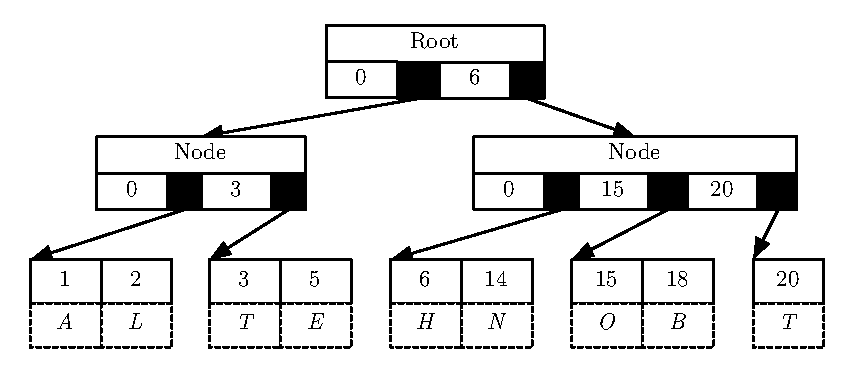
\includegraphics[width=90mm]{diagrams/BPlusTreeImpl.pdf}
 \caption{The same B+ tree as in Figure \ref{fig:bplustree} but with our specific list implementation.}
 \label{fig:bplustreeImpl}
\end{figure}

Figure \ref{fig:bplustree} correctly shows that for each node with $n$ keys there are $n+1$ pointers to sub trees. As it can be seen from both Figure \ref{fig:inductive_data_type} and \ref{fig:bplustreeImpl} we have chosen to deal with this asymmetry by always having a $0$ key in the beginning of each key-pointer list such that every node has $n+1$ key-pointer paris. Another way to represent a node would be to have $n$ key-pointer pairs as well as a start pointer of the type \begin{coqdoccode}\coqdocvar{bplustree} \coqdocvar{b} \coqdocvar{X}\end{coqdoccode}. However, that would give us unnecessary complexity both when writing our primary functions but also when proving theorems about these functions. Even though it is more strongly typed with such a definition we would always have to take care of a start pointer corner case when proving anything about our B+ trees. With our current solution we add a couple of assumptions to our notion of what a valid B+ tree is, to ensure the start pointer is properly handled. This will be explained in the following section. \todo{insert ref}

\paragraph{}
\todo{Write about valid bplus}

\paragraph{}
\todo{Write about appears in...}

\subsubsection{Search}
Our implementation of search does not stray far from the prototypical version described in the background (Section \ref{sec:Background}). It is implemented through 3 functions: $search'$, $find_subtree$, and $search_leaf$. 
\todo{Write about sorted}

\paragraph{}
Both our $insert$ and $search$ are recursive function recursing over a descending parameter $counter$. The reason for introducing this parameter is to serve as a recursion terminator. Because our inductive type for B+-trees consists of a nesting of two inductive datatypes that are not mutually recursive, Coq is unable to reason about instances of $bplustree$ has a recursively decreasing argument. Since a key requirement for recursive Coq functions is that they must contain a decreasing argument, we introduced this notion of a counter that we will decrease by one every time we decent one down to a subtree. If the counter ever reaches $0$, the recursion stops. This means that should the counter ever reach $0$ before we have descended all the way down the tree, a wrong result will be given. To ensure this never happens, we always initialize the counter to the height of the tree.

The reason why initializing the counter to the height of the tree will guarantee that our counter will never reach $0$ before our $insert'$ implementation have descended all the way down to a leaf is simple. Our implementation of $height$ performs 

\subsubsection{Insert}
Since Gallina does not support arrays, the only way to get lookups faster than $O(n)$ is through a tree structure, such as a B+ tree. This would add a large degree of complexity to our proofs, and since running time is not an objective of this project, it has been deemed out of scope.

\paragraph{}
